\begin{figure}
  \centering
  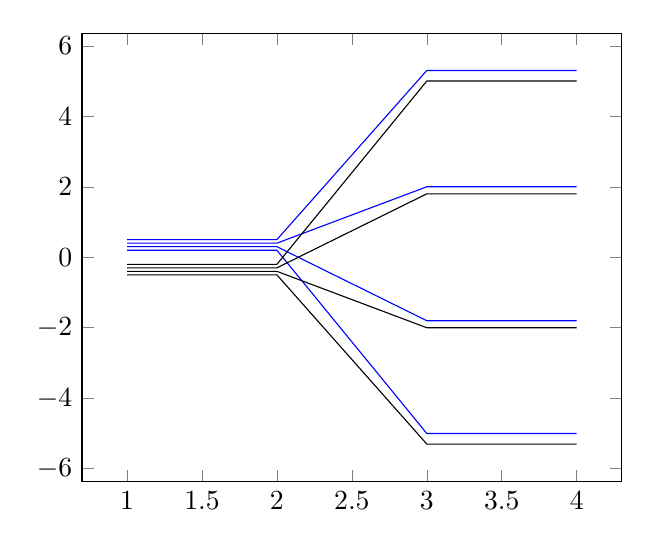
\begin{tikzpicture}
    \begin{axis}
      \addplot [color=blue] coordinates {
        (1, 0.2)
        (2, 0.2)
        (3, -5)
        (4, -5)
      };
      \addplot [color=blue] coordinates {
        (1, 0.3)
        (2, 0.3)
        (3, -1.8)
        (4, -1.8)
      };
      \addplot [color=blue] coordinates {
        (1, 0.4)
        (2, 0.4)
        (3, 2)
        (4, 2)
      };
      \addplot [color=blue] coordinates {
        (1, 0.5)
        (2, 0.5)
        (3, 5.3)
        (4, 5.3)
      };
      \addplot [color=black] coordinates {
        (1, -0.2)
        (2, -0.2)
        (3, 5)
        (4, 5)
      };
      \addplot [color=black] coordinates {
        (1, -0.3)
        (2, -0.3)
        (3, 1.8)
        (4, 1.8)
      };
      \addplot [color=black] coordinates {
        (1, -0.4)
        (2, -0.4)
        (3, -2)
        (4, -2)
      };
      \addplot [color=black] coordinates {
        (1, -0.5)
        (2, -0.5)
        (3, -5.3)
        (4, -5.3)
      };
    \end{axis}
  \end{tikzpicture}
  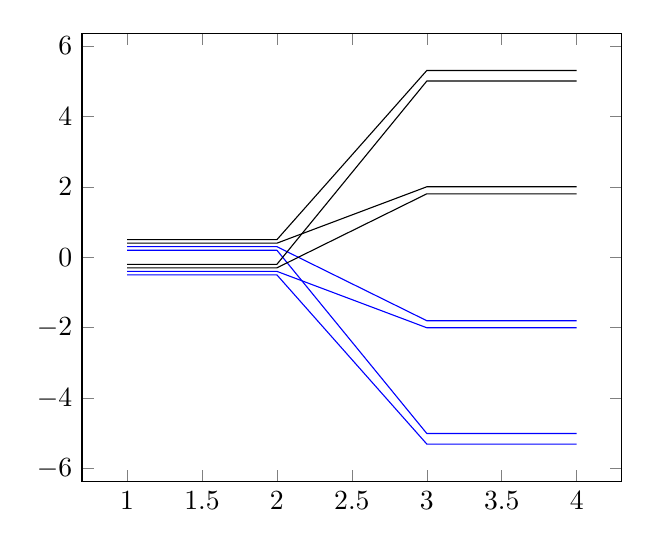
\begin{tikzpicture}
    \begin{axis}
      \addplot [color=blue] coordinates {
        (1, 0.2)
        (2, 0.2)
        (3, -5)
        (4, -5)
      };
      \addplot [color=blue] coordinates {
        (1, 0.3)
        (2, 0.3)
        (3, -1.8)
        (4, -1.8)
      };
      \addplot [color=black] coordinates {
        (1, 0.4)
        (2, 0.4)
        (3, 2)
        (4, 2)
      };
      \addplot [color=black] coordinates {
        (1, 0.5)
        (2, 0.5)
        (3, 5.3)
        (4, 5.3)
      };
      \addplot [color=black] coordinates {
        (1, -0.2)
        (2, -0.2)
        (3, 5)
        (4, 5)
      };
      \addplot [color=black] coordinates {
        (1, -0.3)
        (2, -0.3)
        (3, 1.8)
        (4, 1.8)
      };
      \addplot [color=blue] coordinates {
        (1, -0.4)
        (2, -0.4)
        (3, -2)
        (4, -2)
      };
      \addplot [color=blue] coordinates {
        (1, -0.5)
        (2, -0.5)
        (3, -5.3)
        (4, -5.3)
      };
    \end{axis}
  \end{tikzpicture}
  \caption{A stochastic process, for which algorithms that operate stagewise may yield arbitrarily bad results.
    The first plot shows the partition found by an algorithm which fixes the first stage before considering the second. 
    This yields a tree that is by far inferior to the one obtained by adjusting the tree to all stages at the same time}
  \label{fig:stagewise-failure}
\end{figure}